%% ----------------------------------------------------
\chapter{Testing} \label{Chapter: Testing}


\section{Data Retrieval}



\subsection{Machine Learning Model Test and Training Data}


\section{Data Upload and Storage}

\section{AWS IoT Greengrass / Edge Node Deployment}

\section{Testing Phase of Machine Learning Model with Test Dataset}
\subsection{Data Throughput Strength Classifier}
The trained machine learning model (classifier) is evaluated with the test set which contains 10\% of the data. The performance of the data throughput strength classifier is illustrated in a confusion matrix by making use of the heatmap function available. A classification report is also produced to evaluate the performance of the classifier which displays measurement metrics such as accuracy, recall, precision, and F1-score. 

\subsubsection{k-NN Algorithm with 800 Data Points}
Firstly, the model built with the k-Nearest Neighbour algorithm using the 800 data points is first tested. The confusion matrix for the model is shown in Fig. \ref{fig_cm1}. The diagonal values in the matrix represent the correctly classified data points with respect to their classes. Data points outside of the diagonal values are misclassified points. For example, there are 4 points from the strong data throughput class misclassified under the moderate data throughput class. 

\begin{figure} [ht]
    \centering
    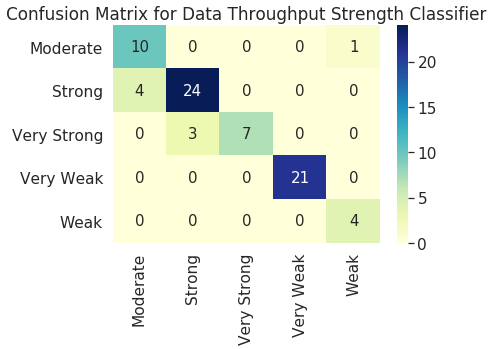
\includegraphics[scale=1.0]{pages/Chapter 5/Chapter 5 images/knn_800.PNG}
    \caption{Confusion matrix of Data Throughput Strength Classifier}
    \label{fig_cm1}
\end{figure}

A classification report for the tested model is shown in Fig. \ref{fig_crknn}. The accuracy achieved by the model is 89\%. The precision, recall and f1-score for each class is also displayed. The support column shows the actual amount of data points that belong to their corresponding classes.   

\begin{figure} [ht]
    \centering
    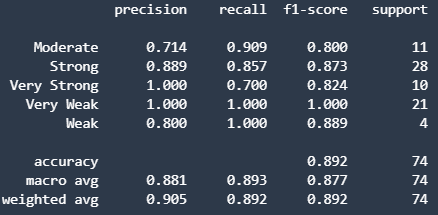
\includegraphics[scale=1.3]{pages/Chapter 5/Chapter 5 images/C_report_knn.PNG}
    \caption{Classification report of the k-NN classifier}
    \label{fig_crknn}
\end{figure}


\subsubsection{k-NN Algorithm with 6000 Data Points}
The confusion matrix is produced for the trained model with the 6000 data points used. The classification report for the tested model is obtained. The accuracy achieved by the model is approximately 99\%. Therefore, the model with a larger data set gives a better overall performance in classifying data.

\begin{figure} [ht]
    \centering
    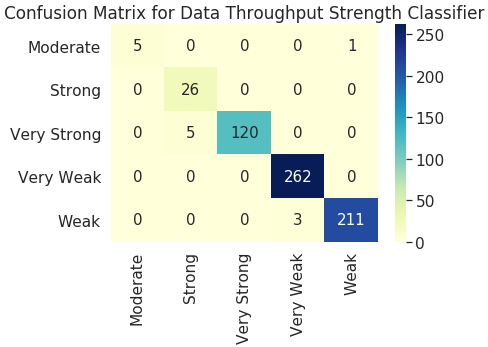
\includegraphics[scale=1.0]{pages/Chapter 5/Chapter 5 images/knn_6k.PNG}
    \caption{Confusion matrix of Data Throughput Strength Classifier}
    \label{fig_cm1}
\end{figure}


\begin{figure} [ht]
    \centering
    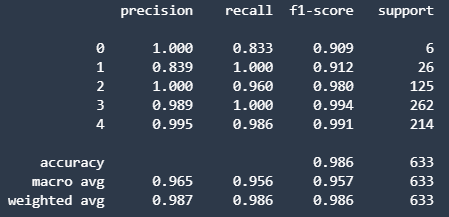
\includegraphics[scale=1.3]{pages/Chapter 5/Chapter 5 images/C_report_knn6k.PNG}
    \caption{Classification report of the k-NN classifier}
    \label{fig_crknn}
\end{figure}

\subsubsection{XGBoost Algorithm with 800 Data Points}

\subsubsection{XGBoost Algorithm with 6000 Data Points}

\begin{figure} [ht]
    \centering
    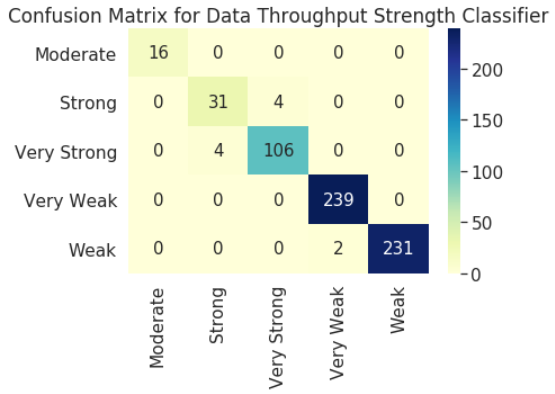
\includegraphics[scale=1.0]{pages/Chapter 5/Chapter 5 images/cm_xgb6k.PNG}
    \caption{Confusion matrix of the XGBoost classifier}
    \label{fig_crknn}
\end{figure}

\begin{figure} [ht]
    \centering
    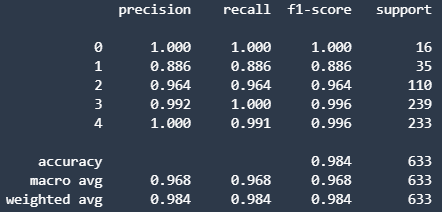
\includegraphics[scale=1.3]{pages/Chapter 5/Chapter 5 images/C_report_xgb6k.PNG}
    \caption{Confusion matrix of the XGBoost classifier}
    \label{fig_crknn}
\end{figure}
\section{Testing Phase of Machine Learning Model with Postman}